

\definecolor{tiffanyblue}{RGB}{129,216,208}
\definecolor{bangdiblue}{RGB}{0,149,182}
\definecolor{kleinblue}{RGB}{0,47,167}
\definecolor{kabuliblue}{RGB}{26,85,153}
\definecolor{purple}{RGB}{138,43,226}
\usepgfplotslibrary{groupplots}
\begin{figure*}[t!]
  \centering
  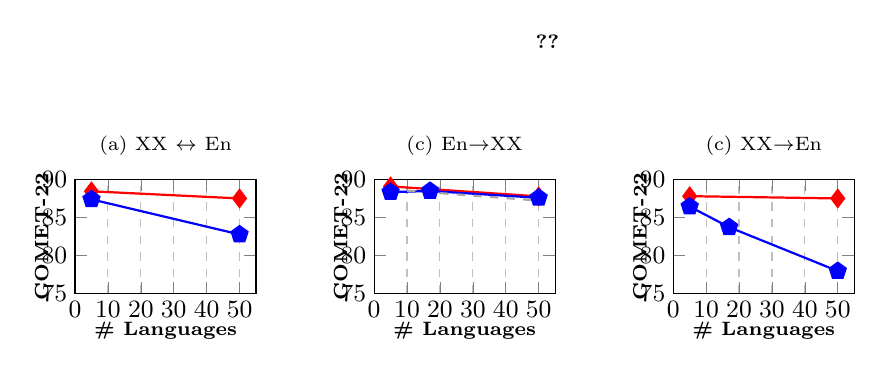
\begin{tikzpicture}
    \pgfplotsset{set layers}
    \scriptsize{
    \begin{groupplot}[
      group style={group size=3 by 1, horizontal sep=1.5cm},
      xmajorgrids,
      grid style={dashed, gray!50},
      width=0.32\textwidth,
      height=.25\textwidth,
      xlabel={\# Languages},
      ylabel={COMET-22},
      xlabel style={font=\bfseries, yshift=0.5em},
      ylabel style={font=\bfseries, yshift=-1.0em},
      yticklabel style={font=\small},
      xticklabel style={font=\small},
      ymin=75, ymax=90, 
      ytick={75, 80, 85, 90},
      xmin=0, xmax=55, 
      xtick={0, 10, 20, 30, 40, 50},
      legend style={
        at={(1.5,-0.25)},
        anchor=north,
        draw=none, fill=none, font=\small, column sep=1ex
      },
      legend columns=-1
    ]

    % Subplot 1: En <-> XX
    \nextgroupplot[title={(a) XX $\leftrightarrow$ En},
    legend to name=namedlegend]
    \addplot[red, mark=diamond*, mark size=3.0pt, thick, mark options={solid, fill=red}] 
      coordinates {(5, 88.46)  (50, 87.52)};
    \addlegendentry{XALMA-13B-Ours}
    % \addplot[orange, mark=triangle*, mark size=3.0pt, thick, mark options={solid, fill=orange}] 
    %   coordinates {(5, 86.90) (17, 81.53) (50, 74.46)};
    % \addlegendentry{ALMA-13B}
    \addplot[blue, mark=pentagon*, mark size=3.0pt, thick, mark options={solid, fill=blue}] 
      coordinates {(5, 87.40) (50, 82.79)};
    \addlegendentry{XALMA-13B}
    

    % Subplot 2: En-XX
    \nextgroupplot[title={(c) En$\rightarrow$XX}]
    \addplot[red, mark=diamond*, mark size=3.0pt, thick, mark options={solid, fill=red}] 
      coordinates {(5, 89.10) (50, 87.79)};
    % \addplot[orange, mark=triangle*, mark size=3.0pt, thick, mark options={solid, fill=orange}] 
    %   coordinates {(17, 83.28) (50, 80.33)};
    \addplot[blue, mark=pentagon*, mark size=3.0pt, thick, mark options={solid, fill=blue}] 
      coordinates {(5, 88.35) (17, 88.50) (50, 87.60)};

    \addplot[thick, dashed, gray!70] 
      coordinates {(5, 88.71) (50, 87.24)};

    
    
    % Subplot 3: XX-En
    \nextgroupplot[title={(c) XX$\rightarrow$En}]
    \addplot[red, mark=diamond*, mark size=3.0pt, thick, mark options={solid, fill=red}] 
      coordinates {(5, 87.82) (50, 87.52)};
    % \addplot[orange, mark=triangle*, mark size=3.0pt, thick, mark options={solid, fill=orange}] 
    %   coordinates { (17, 79.79) (50, 68.60)};
    \addplot[blue, mark=pentagon*, mark size=3.0pt, thick, mark options={solid, fill=blue}] 
      coordinates {(5, 86.45) (17, 83.74) (50, 77.98)};

    %   \addplot[thick, dashed, gray!70] 
    %   coordinates {(5, 87.82) (50, 87.52)};
    % % \node at (0.5,-10.25) {(c) XX-En};

    \end{groupplot}
    }
    % \node[above=0.5cm] at (group c1r1.north) {\ref{namedlegend}};
    \node at (6,3.2) {\ref{namedlegend}};
  \end{tikzpicture}
  \vskip -0.1in
  \caption{Performance comparison between our methods and the baseline on Flores test sets for different translation directions.}
  \label{fig:comparison_scaling_methods_subplots}
\end{figure*}


